% !TeX spellcheck = en_B
% !TeX encoding = UTF-8 %%%These comments just make you look like you know what you're doing
\documentclass[8pt]{beamer}  %%% Specifies the class, with 8pt font size

\usepackage[utf8]{inputenc}
\usetheme[block=fill,progressbar=foot,background=light]{metropolis}     
\usepackage[english]{babel}
\usepackage{csquotes}       
\usepackage[T1]{fontenc}        
\usepackage{booktabs}
\usepackage{pgfgantt}
\usepackage{pifont}
\usepackage{adfbullets}
\usepackage{enumitem}
\usepackage{amsmath}   
\usepackage{tikz}
\usepackage{lipsum}
\usepackage{amssymb}
\usepackage{amsfonts}
\usepackage{mathrsfs}   
\usepackage{graphicx}
\usepackage{adjustbox}
\usepackage{varioref}
\usepackage{probsoln}
\usepackage{attachfile2}
\usepackage{pgfplots}
\pgfplotsset{compat=newest}
\usepackage[]{hyperref} 
\graphicspath{{Graphics/}}
\usepackage{multirow,array}
\usepackage{colortbl}
\definecolor{aa}{RGB}{255, 124, 0}
\definecolor{cc}{RGB}{230, 230, 230}    
\usebackgroundtemplate{%
\tikz[overlay,remember picture]{\node[scale=80,opacity=0.03, at=(current page.south east)] {\adfbullet{9}};}}
  
\date[\today]{\today}

\usepackage{comment}
\usepackage{varwidth}

\newcommand{\mat}[4]{\left(\begin{array}{cc} #1 & #2 \\ #3 & #4 \\ \end{array}\right)}
\newcommand{\Q}{\mathbb{Q}}
\newcommand{\R}{\mathbb{R}}
\newcommand{\Z}{\mathbb{Z}}
\newcommand{\sol}[2][+]{
	\tikz[baseline]{\node[color=aa,fill=cc,rectangle,draw,anchor=base] {  {\onslide<#1->{#2}}  };}
}

\usetikzlibrary{positioning}
\usetikzlibrary{tikzmark}
\usetikzlibrary{shadings}
\usetikzlibrary{through}

\def\height{0.8cm}
\def\width{1.2cm}
\newcommand{\keynode}[6]{\node[minimum height=\height,minimum width=\width,draw,rectangle,color=aa,fill=cc] (#3) at (#1,#2) {};
	\node[rectangle,minimum height=\height/2,minimum width=\width,above,color=aa] at (#3) {#3};
	\node[draw,rectangle,minimum height=\height/2,minimum width=\width/3,below,color=aa,fill=cc,inner sep =0cm] at (#3) {\footnotesize#4};
	\node[draw,rectangle,minimum height=\height/2,minimum width=\width/3,below,xshift=\height/2,color=aa,fill=cc,inner sep=0cm] at (#3) {\footnotesize#5};
	\node[draw,rectangle,minimum height=\height/2,minimum width=\width/3,below,xshift=-\height/2,color=aa,fill=cc,inner sep=0cm] at (#3) {\footnotesize#6}; }

\newenvironment{gantt}[3]{\begin{ganttchart}[#1,bar height=.6,bar top shift=.2,title/.style=  {draw=none},y unit chart=0.6cm,y unit title = 0.6cm,include title in canvas=false,group/.append style={draw=black,dashed},bar/.append style={fill=aa},inline,hgrid=true,Float1/.style={bar/.append style={fill=none,dashed},bar height=.8,bar top shift=0.1}]{#2}{#3}}{\end{ganttchart}}

\newenvironment{nicetable}[1]{\setlength\arrayrulewidth{0.5mm}
			\arrayrulecolor{white}
			\begin{tabular}{#1}}{\end{tabular}}
		
\setlist[itemize,1]{label={\color{aa}\huge\adfbullet{9}}}
\setlist[itemize, 2]{label={\color{aa}\large\adfbullet{9}}}

\newcommand\reshist{}
\def\reshist(#1)#2(#3)#4(#5)%
{\draw (axis cs:#1) rectangle (axis cs:#3) node [midway] {#5};} %%%adds the general preamble

\title{{\color{aa}\Huge\adfbullet{9}}Unleashing Algebraic Metaprogramming in Julia with Metatheory.jl } %%%Title and subtitle
\subtitle{Alessandro Cheli, University of Pisa - Philip Zucker, Draper Labs \\ \small{(a.cheli6@studenti.unipi.it - philzook58@gmail.com)}} %%%This embeds the tikz source code into the resulting pdf...
\date{}

\usepackage{multicol}
\usepackage{jlcode}
\usepackage{listings}
\usepackage{biblatex}
\newcommand{\MYhref}[3][blue]{\href{#2}{\color{#1}{#3}}}%

\bibliography{biblio.bib}

\begin{document}

% ========================================================================


\frame{\titlepage} %%%Makes titlepage

\setlength{\abovedisplayskip}{0pt}
\setlength{\belowdisplayskip}{0pt}
\setlength{\abovedisplayshortskip}{0pt}
\setlength{\belowdisplayshortskip}{0pt}  %%%Compresses math


% ========================================================================

\begin{frame}{Metatheory.jl}   %%%Frame with title

\begin{multicols}{2}
Metatheory.jl \footfullcite{Cheli2021} is a general purpose metaprogramming library for Julia, taking advantage of the language reflection to bridge the gap between symbolic mathematics, abstract interpretation, equational reasoning, optimization, composable compiler transforms and homoiconicity. At its core sits \textit{e-graph rewriting}, a fresh approach to term rewriting achieved through an equality saturation algorithm.

\textcolor{blue}{\href{https://github.com/0x0f0f0f/Metatheory.jl}{https://github.com/0x0f0f0f/Metatheory.jl}}

\columnbreak

\begin{figure}
    \centering
    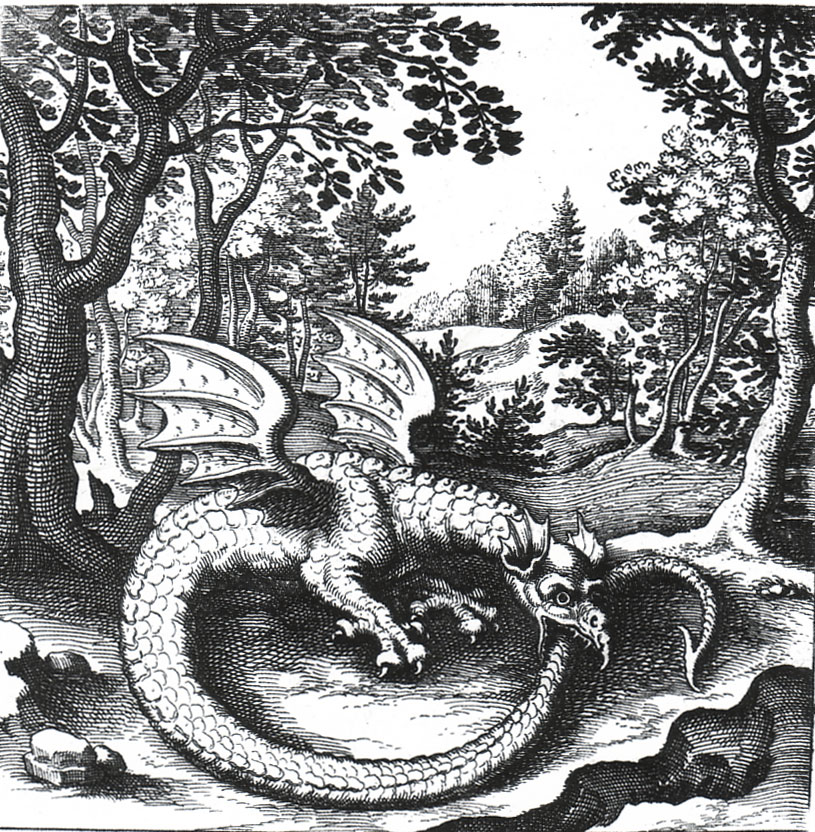
\includegraphics[width=0.4\textwidth]{dragon.jpg}
    \label{fig:my_label}
\end{figure}


\end{multicols}

\end{frame}

% ========================================================================


\begin{frame}{What can we do with Metatheory.jl?} % What can we do with metatheory?

E-Graphs + Julia = 

\begin{itemize}
    \item General purpose equational term rewriting on custom types!
    \item High-level compiler transforms
    \item Flexible symbolic mathematics
    \item Custom code optimizers using equational theories
    \item Flux.jl model optimizers\footfullcite{yang2021equality}
    \item DPLL(T) Theorem Proving\footfullcite{de2008z3}
    \item Symbolic regression algorithms
    \item Floating point error auto fixers (\MYhref{https://github.com/herbie-fp/egg-herbie}{see here})
\end{itemize}

\end{frame}



\begin{frame}{Equations Are Good}  

Supporting bidirectional (\textit{equational!}) rules in term rewriting opens up a world of opportunities.

%I'm just getting stuff typed out. We should discuss what actually goes where
%Equations and equational reasoning are everywhere

Engineering \& Physics
\begin{itemize}
    \item plus, times, cos, sin, exp. $\cos(x)^2 + \sin(x)^2 = 1$ 
    \item integrals, derivatives e.g. $\int x ^ n dx = \frac{x^ {n + 1}}{n} $
    \item matrix and vector algebra e.g. $(A \otimes B) \cdot (C \otimes D) = (A \cdot C) \otimes (B \cdot D)$
    \item commutators and operators $a_i a_j^\dagger - a_j^\dagger a_i = \delta_{ij}$
\end{itemize}
Maths 
\begin{itemize}
   \item Algebraic structures such as Groups $a^2 = b^2 = (ab)^2 = e$
   \item Category theory $f \cdot id_A = f$
\end{itemize}

Computer Science
\begin{itemize}
   \item Stream Fusion \texttt{map f . map g = map (f . g)} 
   \item Compiler Optimizations  \texttt{15 * x = x << 4 - 1} 
   \item Query Optimization
\end{itemize}
\end{frame}


% ========================================================================



\begin{frame}{Classical Rewriting}
\begin{itemize}
\item Mathematica, Maxima, SymPy, Symbolics.jl
\item Term rewriting is typically destructive and \textit{forgets} the matched left-hand side.
\item Equations are oriented (unnaturally?) in one direction.
\item Some rules are obviously good as simplifications.  $\cos(x)^2 + \sin(x)^2 = 1$ 
\item Apply rules in arbitrary or controlled order - Local minima and looping
\item Confluent and terminating rewrite systems - You're golden \footfullcite{dershowitz1993taste}
\item What about non obviously oriented equations? $(a + b) + c = a + (b + c)$
\end{itemize}
\end{frame}

% ================================================================
% Maybe we should cut this?
\begin{frame}[fragile]{E-Graph}

% Define E graphs

% is the first ever implementation of term rewriting through equality saturation on the e-graph %data structure. The \MYhref{https://dl.acm.org/doi/pdf/10.1145/3434304}{egg paper} elegantly % describes the algorithm and the underlying data structure.
\begin{itemize}
\item \MYhref{https://egraphs-good.github.io/}{egg} \footfullcite{egg} - e-graphs implemented in Rust.
%\item First ever implementation of general purpose term rewriting through e-graphs (2021)
\end{itemize}


\begin{figure}
    \centering
    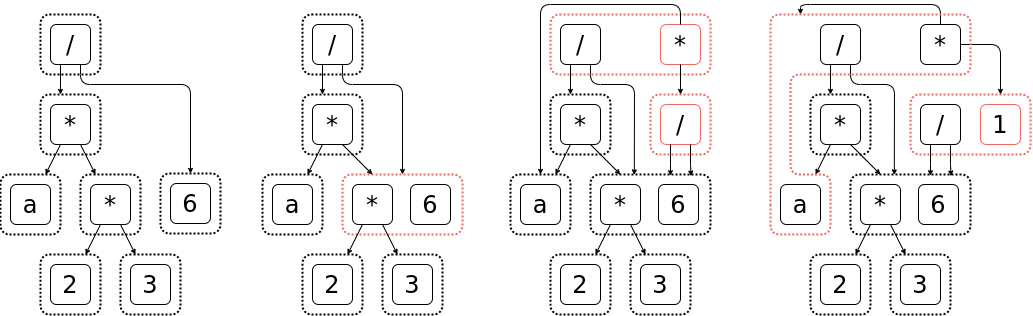
\includegraphics[width=0.8\textwidth]{egraphs.png}
    \caption{The four depicted e-graphs represent the process of equality saturation for the equivalent ways to write $a * (2 * 3) / 6$. The dashed boxes represent equivalence classes, and regular boxes represent e-nodes.}
    \label{fig:egraph}
\end{figure}

\end{frame}



% ================================================================
 % E-Graphs 101
\begin{frame}{The Path to the E-Graph}
% note: pictures would be great here.
\begin{itemize}
\item Non-destructive rule application - copy everything
\item Conceptually egraph is similar to fast data structure for sets of trees.
\item Share subtrees if you can
\item Share parents if you can
\item Bipartite graph of ENodes and EClasses
\item Union-Find and Hash Cons
% \item Propagate equalities upwards - parent pointers $a = b \rightarrow f(a) = f(b)$

% Actually define an egraph
\end{itemize}

\end{frame}

\begin{frame}{Why Julia?}   %%%Frame with title

Julia \footfullcite{bezanson2017julia}:

\begin{itemize}
    \item is high-level, easy to learn
    \item is performant
    \item has excellent LISP-like metaprogramming and reflective capabilities
    \item has an excellent high-level dynamic type system
    \item supports generation and manipulation of programs as first-class values
    \item has an excellent package ecosystem for real world use cases
\end{itemize}

\end{frame}


% Nonintuitive properties of egraphs / Gotchas.
% it would be good to have more demos if possible
% ========================================================================




\begin{frame}[fragile]{A Sketch of an E-Graph in Julia}
    % put julia code of data structures here.
\begin{jllisting}
struct ENode
    head::Symbol
    args::EClassId
end
struct EClass
    members::Set{ENode}
end
struct EGraph
    memo::Dict{ENode, EClassId}
    classes::Dict{EClassId,EClass}
    equiv::IntDisjointSet 
end
\end{jllisting}
\end{frame}


\begin{frame}{Equality Saturation}
    Given a starting e-graph $g$, a set of rewrite rules $t$ and an iteration limit $n$:
    \begin{itemize}
        \item For each rule in $t$, search through the e-graph for l.h.s.
        \item For each match produced, apply the rewrite
        \item Do a bottom-up traversal of the e-graph to rebuild the \textit{congruence closure} 
        \item If the e-graph hasn't changed from last iteration, it has \textbf{saturated}
        \item Loop at most $n$ times. 
    \end{itemize}
    
    Knowing if an expression with a set of rules saturates an e-graph or never terminates is still \textit{an open research problem}.
    
\end{frame}


% ================================================================






% ========================================================================

\begin{frame}[fragile]{What is so cool about e-graphs?}   %%%Frame with title

\begin{itemize}
    \item When to apply which rewrite? \textit{Phase ordering problem}
    \item Apply all rewrites simultaneously? Keep history? \textit{Exponential space and time!}
    \item \textbf{Equality saturation} + \textbf{E-Graphs} = \textbf{E-Graph Rewriting}.
    \item $\implies$ no more phase ordering problem 
    \item $\implies$ bidirectional equational rules for free! 
\end{itemize}

% Too much text for slide

With \textit{e-graph rewriting}  Here's an example rewrite system


\begin{jllisting}
using Metatheory
using Metatheory.Classic
@metatheory_init ()

th = @theory begin
    a + a => 2a     # this rule is ok! 
    a + b => b + a  # causes loops in classical rewriting
    0 + a => a
end 

\end{jllisting}


\end{frame}

% ========================================================================

\begin{frame}[fragile]{Classical Rewriting vs E-Graph Rewriting}   %%%Frame with title

\begin{itemize}
    \item Rule \texttt{a + b => b + a} causes an infinite rewrite loop
    \item User reasoning and rewriting strategies are required to make this terminate!
\end{itemize}

\begin{jllisting}
using Metatheory.Classic
expr = :(x + 0)
rewrite(expr, th)
\end{jllisting}

Result will be \texttt{:(x + 0)}

Using \textit{e-graph} rewriting with equality saturation, the problem is avoided.

\begin{jllisting}
using Metatheory.EGraphs
expr = :(x + 0)
g = EGraph(expr)
saturate!(g, th) # runs equality saturation
extract!(g, astsize) # extract the shortest expression from the e-graph g
\end{jllisting}

Result will be \texttt{:x}


\end{frame}

% ========================================================================



% ========================================================================


% ================================================================

% TODO extraction

% \begin{frame}{Schedulers}

% Applying every rule every iteration is \textit{expensive!}. We can limit the search space of applicable rules at every iteration. This technique is called scheduling in egg.

% Exponential Backoff Scheduling:

% \begin{itemize}
%     \item If a rule produced too many matches (configurable treshold $t$)
%     \item Ban the rule search for a number of iterations $n$
%     \item After $n$ iterations have passed, lift the ban and set $n=2n$, $t=2t$. 
%     \item Proceed to next iteration.
% \end{itemize}

% Scored Exponential Backoff Scheduling (New in Metatheory.jl):

% \begin{itemize}
%     \item Same as exponential backoff
%     \item Computes a \textit{measure of complexity}\footnotemark of the l.h.s. and r.h.s. of rules.
%     \item Don't ban rules that reduce the complexity!
%     \item Decrease $t$ and increase the ban time $n$ of rules that increase complexity.
% \end{itemize}

% \footnotetext[7]{The measure of complexity can be arbitrary, an example can be the AST size of the rule's lhs and rhs.}

% \end{frame}





% ================================================================

\begin{frame}[fragile]{Symbolics.jl}

Metatheory.jl can be used to rewrite Symbolics.jl expressions. This has proved really useful for optimization tasks:
In \footfullcite{gowda2021high} we developed a set of equality rules and a cost function to generate equivalent Symbolics.jl expressions which are computed in fewer CPU cycles. We tested against a 1122 ODE model of B Cell Antigen Signaling and simplified the 24388 terms using Symbolics.jl+Metatheory.jl. The generated code accelerated from $15.023\mu s$ to $7.372\mu s$ per execution, halving the time required to solve the highly stiff ODEs.

\begin{jllisting}
theory = @methodtheory begin
    a * x == x * a
    a * x + a * y == a*(x+y)
    -1 * a == -a
end
\end{jllisting}

\end{frame}

\begin{frame}{Symbolics.jl}
    
\begin{figure}
    \centering
    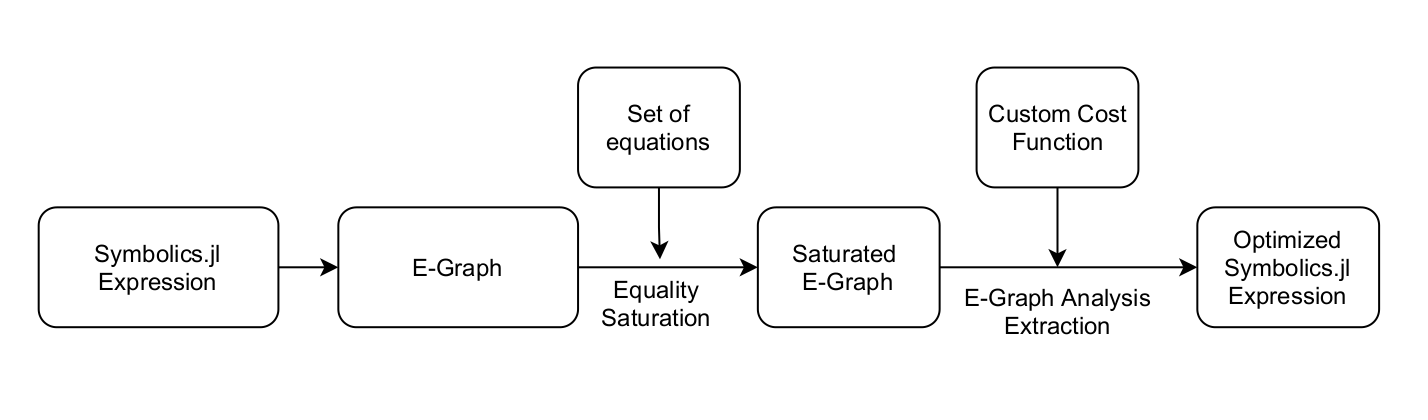
\includegraphics[width=\textwidth]{Symbolics.png}
    \caption{Pipeline of Symbolics.jl expression optimization}
    \label{fig:my_label}
\end{figure}

We are developing TermInterface.jl, a package for a shared interface that represents
symbolic expressions. To rewrite on arbitrary expression types with Metatheory.jl, it will be necessary 
to implement a few methods from this interface (\texttt{isterm, arity, gethead, getargs, similarterm...})

\end{frame}

% ================================================================


\begin{frame}[fragile]{Fibonacci with SymbolicUtils.jl vs Metatheory.jl}

SymbolicUtils.jl \vspace{-0.4cm}
\begin{jllisting}
@syms fib(x::Int)::Int

const rset = [
    @rule fib(0) => 0
    @rule fib(1) => 1
    @rule fib(~n) => fib(~n - 1) + fib(~n - 2)
] |> Chain |> Postwalk |> Fixpoint

compute_fib(n) = rset(fib(n))
\end{jllisting}
Metatheory.jl \vspace{-0.4cm}
\begin{jllisting}
const fibo = @theory begin
    x::Int + y::Int |> x+y
    fib(n::Int) |> (n < 2 ? n : :(fib($(n-1)) + fib($(n-2))))
end;

function compute_fib(n)
    g = EGraph(:(fib($n)))
    saturate!(g, fibo, SaturationParams(timeout=7000, scheduler=SimpleScheduler))
    extract!(g, astsize)
end
\end{jllisting}

\end{frame}
 

\begin{frame}[fragile]{vs. Fibonacci with Metatheory}
\begin{figure}
    \centering
    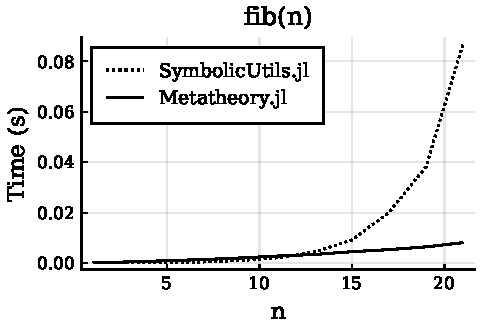
\includegraphics[width=0.5\textwidth]{fib.pdf}
    \caption{Benchmark of Fibonacci Sequence computation of SymbolicUtils.jl against Metatheory.jl. MT achieves implicit memoization of computation with e-graphs!}
    \label{fig:my_label}
\end{figure}
\end{frame}

% TODO Superinterpreter?

% ================================================================

%\begin{frame}{Category Theory}

%\begin{itemize}
%    \item Categories - A powerful abstraction. LA, RA, functional programs can be modeled
%    \item Generalized Algebraic Theories (GATs) -  Equational reasoning on types and terms
 %   \item Guarded E-matching $(A \otimes B) \cdot (C \otimes D) = (A \cdot C) \otimes (B \cdot D)$
 %   \item Internalized type derivation
 %   \item Open Question: 
 %   \item Future direction: proofs, automating translation from Catlab
%\end{itemize}

%\end{frame}

% ================================================================

\begin{frame}{Category Theory}

We have experimented with

\begin{itemize}
    \item Categories - A powerful abstraction. LA, RA, functional programs can be modeled
    \item Rewriting Catlab.jl expressions using Metatheory.jl
    \item GATs\footnote{Generalized Algebraic Theories}-  Equational reasoning on types and terms
    
   % \item Converting Catlab.jl theory axioms to Metatheory.jl rules 
    \item Alternative algebraic encodings for GATs in pure Julia
    \item Proving equality of expressions over theories by e-graph rewriting
\end{itemize}
One possible encoding\footnote{\MYhref{https://www.philipzucker.com/metatheory-progress/}{https://www.philipzucker.com/metatheory-progress/}}:

\begin{itemize}
    \item Guarded E-matching $(A \otimes B) \cdot (C \otimes D) = (A \cdot C) \otimes (B \cdot D)$
    \item Internalized type derivation
    \end{itemize}
    
Is this the right way to go?


%\tiny{\MYhref{blog_post}{https://www.philipzucker.com/metatheory-progress/}
% \tiny{\\Metatheory.jl takes around 0.04364s, KnuthBendix.jl fails!}
%The process of mechanizing categorical reasoning for Catlab.jl is still in an early stage. We still need

%\begin{itemize}
%    \item A system to infer which rules are useful to apply and which rule are not (scheduler)
%    \item Better encodings of categorical expressions to be used for rewriting
%    \item A precise algorithm that provides proofs
%\end{itemize}


\end{frame}

% ================================================================

\begin{frame}[fragile]{Going Faster than Knuth-Bendix}

Hurwitz groups of type $(2,3,7, n)$. Is an expr. equal to $\varepsilon$? Thanks to Marek Kaluba (\MYhref{https://github.com/kalmarek/}{@kalmarek})

\begin{jllisting}
rep(x, op, n::Int) foldl((x, y) -> :(($op)$x, $y)), repeat([x], n))

T = [
    @rule a * :ε => a # identity element
    @rule :ε * a => a
    @rule a * (b * c) => (a * b) * c # associativity
    @rule (a * b) * c => a * (b * c)
    @rule :b*:B => :ε # inverses
    @rule :a*:a => :ε
    @rule :b*:b*:b => :ε
    @rule :B * :B => :B
    RewriteRule(Pattern(rep(:(:a*:b), :*, 7)), Pattern(:(:ε)))
    RewriteRule(Pattern(rep(:(:a*:b*:a*:B), :*, 12)), Pattern(:(:ε)))
]


g = EGraph(:(a*b* a*a*a * b*b*b * a * B*B*B*B * a))
params = SaturationParams(timeout=8, scheduler=BackoffScheduler)
@timev saturate!(g, G, params)
@test extract!(g, astsize) == :ε
\end{jllisting}

\tiny{\MYhref{https://www.heldermann-verlag.de/gcc/gcc02/gcc028.pdf}{https://www.heldermann-verlag.de/gcc/gcc02/gcc028.pdf}
\tiny{\\Metatheory.jl takes around 0.04364s, KnuthBendix.jl fails!}
}

\end{frame}

\begin{frame}{Other Experiments}
    You can find other experiments in the \texttt{tests/} folder in the Metatheory.jl source code!
    \begin{itemize}
        \item $\lambda$-calculus partial evaluator
        \item Propositional logic/SAT solver
        \item WHILE-language interpreter/superinterpreter with reversible computations
    \end{itemize}
\end{frame}

% ================================================================



% ================================================================

% \begin{frame}{Not all roses}

% \begin{itemize}
%     \item Metatheory.jl is still quite slower than egg
%     \item Equality saturation is a memory intensive process
%     \item Debugging rewrites is hard
%     \item The interface for rewriting on custom types is not yet stable
%     \item The search process can get lost in useless rewrites
% \end{itemize}

% \end{frame}

% ================================================================

\begin{frame}{Future directions}

Internals:

\begin{itemize}
    \item A shared interface package for interoperability between symbolic packages 
    \item Better pattern matching
    \item Smarter scheduler algorithms for fast, more efficient saturation.
    \item Defining and implementing and algorithm for human-readable (but verifiable) proof paths in e-graphs (Oliver Flatt has been working on this)
    \item Better debugging and logging utilities. (What caused this failure? Which rules are problematic in a system?)
\end{itemize}

Experiments and Use Cases:
\begin{itemize}
    \item Array Symbolics with Symbolics.jl! 
    \item Optimizing the Julia IRs
    \item Optimizing Flux.jl deep learning models
    \item Optimizing quantum circuits for Yao.jl (Thanks to Chen Zhao)
\end{itemize}
\end{frame}

\begin{frame}{}

\Huge{Thank You!}

\end{frame}

% ================================================================

% ================================================================


% \begin{frame}{Egg - Why E-Graphs}   %%%Frame with title

% \MYhref{https://egraphs-good.github.io/}{egg} \footfullcite{egg} is the first ever implementation of term rewriting through equality saturation on the e-graph data structure. The \MYhref{https://dl.acm.org/doi/pdf/10.1145/3434304}{egg paper} elegantly describes the algorithm and the underlying data structure.
% The core egg library provides high-performance, flexible e-graphs implemented in Rust.

% Philip first posted the \MYhref{https://egraphs-good.github.io/}{egg} paper on the Julia Zulip chat server, on the \texttt{\#symbolic-programming channel} and decided to re-implement the algorithms in Julia.
% Alessandro then made it support homoiconic Julia expressions and turned it into a feature-complete Julia package.
% \end{frame}

% ========================================================================




% \begin{frame}{Boxes}
% 	There are three commonly used boxes.
	
% 	\begin{definition}
% 	This is a \textbf{definition box}, it can be helpful to put the word being defined into bold text.
% 	\end{definition}
	
% 	\begin{problem}
% 	        This is a problem box. With some displayed math...
% 	        \[y=x^2\]
% 	\end{problem}
	
% 	\begin{solution}<2->
% 	This is a solution which only appears on the next slide.
% 	\end{solution}
	
% 	\begin{solution}<3->
% 	Appears even later!
% 	\end{solution}

% \end{frame}

% \begin{frame}{The sol command}

% The first time you use \sol{it doesn't cover it up}.

% However the second time \sol{it does}.

% You can put math inside it, $5x+4x=$ \sol{$9x$}

% And you can use it inside a math environment:

% \begin{align*}
%     y &= \sol{5} \\
%     x &= \sol{$x^2$} \\
%     xy &= \sol{$5x^2$}
% \end{align*}

% But this will throw up some errors, but still compile.

% \end{frame}

% \begin{frame}{columns}
%     \begin{columns}
%     \begin{column}{.5\linewidth}
%     Columns can be very useful.
%     \end{column}
%     \begin{column}{.5\linewidth}
%     To display info side by side.
%     \end{column}
%     \end{columns}
%         \begin{columns}[T] %%%Aligned at the top!!!
%     \begin{column}{.5\linewidth}
%     \begin{problem}
%             You can even put boxes inside the columns to save space.
%     \end{problem}
%     \end{column}
%     \begin{column}{.5\linewidth}
%     \begin{solution}<2->
%     With a solution.
%     \end{solution}
%     \end{column}
%     \end{columns}
    
% \begin{definition}
% \noindent
% \begin{minipage}{.4\linewidth}
% Using columns inside boxes is best achieved with minipages.
% \end{minipage}%
% \begin{minipage}{.6\linewidth}
% \begin{center}
% \colorbox{cc!30}{
% \begin{nicetable}{cc|ccc}
% \multicolumn{2}{c}{} & \multicolumn{3}{c}{Player $2$}\\
% \multicolumn{1}{c}{} &  & $X$  & $Y$ & $Z$ \\ \cline{2-5}
% \raisebox{0.0cm}{\multirow{3}*{\rotatebox{90}{Player $1$}}}  & $P$ & $4$ & $2$ & $2$ \\
% & $Q$ & $-3$ & $5$ & $1$ \\
% & $R$ & $2$ & $-1$ & $3$ \\
% \end{nicetable}}
% \end{center}
% \end{minipage}
% \end{definition}
% \end{frame}







% \begin{frame}{The tikzmarknode command}

%     \alert{Useful when annotating equation}
    
%     Use it anywhere to create a node named anything that you can refer back to later. Also compiles but with errors...
    
% 	\begin{flalign*}
% 		\text{Maximise} && P &= V-3 && \\
% 		\text{Subject to} && V -6p-4q + s_1 &= 0 && \\
% 				  && V -p-7q + s_2 &= 0 && \\
% 				  && \tikzmarknode{A}{p + q + s_3} &= 1 &&
% 	.\end{flalign*}

% \begin{tikzpicture}[overlay,remember picture]
%     \draw[color=aa,<-] (A) --++ (1,-1) node[fill=cc] {The annotation $x^2$};
% \end{tikzpicture}

% \end{frame}

% \begin{frame}{Tables}

% \begin{center}
% \colorbox{cc!30}{
% \begin{nicetable}{c|cccccc|c}
% $P$ & $v$ & $p$ & $q$ & $s_1$ & $s_2$ & $s_3$ & RHS \\ 
%   \hline
% 1 & $-1$ & $0$ & $0$ & 0 & 0 & 0 & $-3$   \\ 
%   \hline
% 0 & 1 & $-6$ & $-4$ & 1 & 0 & 0 & 0 \\ 
%   0 & 1 & $-1$ & $-7$ & 0 & 1 & 0 & 1  \\ 
%   0 & 0 & $1$ & 1 & 0 & 0 & 1 & 1 \\ 
% \end{nicetable}}
% \end{center}

% Tikz pictures, as well as tables, basically everything can be shrunk with the adjust box command. You can specify max width, max height, width height etc.

% \centering
% \adjustbox{max width=4cm}{
% \colorbox{cc!30}{
% \begin{nicetable}{c|cccccc|c}
% $P$ & $v$ & $p$ & $q$ & $s_1$ & $s_2$ & $s_3$ & RHS \\ 
%   \hline
% 1 &\boxed{$-1$} & $0$ & $0$ & 0 & 0 & 0 & $-3$   \\ 
%   \hline
% 0 & 1 & $-6$ & $-4$ & 1 & 0 & 0 & 0 \\ 
%   0 & 1 & $-1$ & $-7$ & 0 & 1 & 0 & 0  \\ 
%   0 & 0 & $1$ & 1 & 0 & 0 & 1 & 1 \\ 
% \end{nicetable}}
% }

% \end{frame}


% \begin{frame}[shrink=60]{The shrink command, automatically shrinks to fit on page, but is helpful to give a number so it knows how much horizontal space it has.}
% This is the contents.

% \lipsum

% \begin{problem}
%         \lipsum
% \end{problem}

% \end{frame}


% \begin{frame}{The onslide}
%     Can be used on anything but really cool with tikz pictures.
%                 \centering
% \adjustbox{max width=.8\textwidth}{
% \def\complex{(0,0) ellipse (7cm and 6cm)} %%%%These can be used as variables
% \def\real{(0,0) ellipse (6.5cm and 3.5cm)}
% \def\algebraic{(1.7,0) circle (5cm)}
% \def\imag{(1.3,-4.7) ellipse (2.2cm and 1cm)}
% \def\int{(2.9,-0.6) ellipse (2.6cm and 2.3cm)}
% \def\whole{(2.9,-0.7) ellipse (2.1cm and 1.6cm)}
% \def\count{(2.9,-0.9) ellipse (1.3cm and 1cm)}
% \begin{tikzpicture}
%         %%Complex%%%%%%%%%%%%%%%%%%5
%         \onslide<2->{\filldraw[orange,fill opacity=0.1] \complex;
%         \node[color=orange] at (0,5.5) {Complex Numbers};
%         \node[color=orange] at (-4,4.2) {$\pi+3i$};
%         \node[color=orange] at (-5,3.2) {$e-\pi i$};}
%         %%%%%%Real%%%%%%%%%%%%%5
%         \onslide<3->{\filldraw[green,fill opacity=0.1] \real;
%         \node[color=green] at (0,3) {Real Numbers};}
%         %%%%Transcendental%%%%%%%%%%5
%         \onslide<4->{\node[color=green,align=left] at (-5,0.3) {Transcendental \\ Numbers};
%         \node[color=green] at (-6,-0.5) {$\pi$};
%         \node[color=green] at (-5.3,-1) {$e$};}      
%         %%%%%%%Irrational and real%%%%%%
%         \onslide<5->{\node[color=green] at (-2.9,2.3) {Irrational Numbers};
%         \node[color=green] at (2.9,2.3) {Rational Numbers};
%         \draw[color=green] (0,-3.5) -- (0,2.5);
%         \node[color=green] at (-1.7,1.4) {$\sqrt{2}$};
%         \node[color=green] at (-2.6,-0.3) {$-\sqrt{5}$};                
%         \node[color=green] at (-1.3,-2.2) {$\sqrt[3]{26}$};
%         \node[color=green] at (0.9,1.6) {$\frac{2}{3}$};                
%         \node[color=green] at (5.7,0.7) {$\frac{97}{32}$};}
%         %%%%%Algebraic%%%%%%%%%%
%         \onslide<6->{\filldraw[blue,fill opacity=0.1]  \algebraic;
%         \node[color=blue] at (1.7,4.5) {Algebraic Numbers};
%         \node[color=blue] at (3.7,3.9) {$9+5i$};
%         \node[color=blue] at (4.6,3.1) {$1+i$};}
%         %%%%%Imag%%%%%%%%%%%%%%%
%         \onslide<7->{\filldraw[purple,fill opacity=0.1]  \imag;
%         \node[color=purple] at (1.3,-4.3) {\footnotesize Pure Imaginary Numbers};
%         \node[color=purple] at (-0.5,-5) {$e i$};
%         \node[color=purple] at (0.5,-5.3) {$\pi i$};
%         \node[color=purple] at (0.8,-4.6) {$i$};
%         \node[color=purple] at (2.0,-4.7) {$5 i$};}
%         %%%%%Int%%%%%%%%%%%%%
%         \onslide<8->{\filldraw[color=blue, fill opacity=0.1] \int;
%         \node[color=blue] at (2.9,1.2) {Integers};
%         \node[color=blue] at (0.9,0.4) {$5$};
%         \node[color=blue] at (2.6,-2.6) {$-99$};}
%         %%%%%5Whole%%%%%%5
%         \onslide<9->{\filldraw[color=blue, fill opacity=0.1] \whole;
%         \node[color=blue] at (2.9,0.3) {Whole Numbers};
%         \node[color=blue] at (4.5,-0.6) {$0$};}
%         %%%%%%%%%%Count%%%%%%%%%
%         \onslide<10->{\filldraw[color=blue, fill opacity=0.1] \count;
%         \node[color=blue,align=center] at (2.9,-0.5) {Counting \\ Numbers};
%         \node[color=blue] at (2.2,-1.2) {$1$};
%         \node[color=blue] at (2.8,-1.6) {$2$};
%         \node[color=blue] at (3.4,-1.3) {$99$};}
% \end{tikzpicture}}

% \end{frame}

\end{document}
